\documentclass[12pt]{report}
\usepackage[utf8]{inputenc}
\usepackage[T1]{fontenc}
\usepackage[french]{babel}
\usepackage{geometry}
\usepackage{setspace}
\usepackage{titlesec}
\usepackage{graphicx}
\usepackage{hyperref}
\usepackage{lipsum}
\usepackage{fancyhdr}
\usepackage{color}
\usepackage{float}
\usepackage{pdflscape}
\usepackage{graphicx}

\geometry{a4paper, margin=2.5cm}
\setstretch{1.2}

\titleformat{\chapter}[hang]{\normalfont\LARGE\bfseries}{\thechapter.\ }{0pt}{}
\titlespacing*{\chapter}{0pt}{1em}{1em}

\makeatletter
\renewcommand{\chapter}{\@startsection{chapter}{0}{\z@}
  {-3.5ex \@plus -1ex \@minus -.2ex}
  {2.3ex \@plus.2ex}
  {\normalfont\LARGE\bfseries}}
\makeatother

\title{Analyse et Classification de Scripts de Films}
\author{Alexis LE TRUNG, Aniss OUTALEB, Pierre CHHIENG, Rick GAO}
\date{Mai 2025}

\begin{document}

% Page de garde
\begin{titlepage}
    \begin{center}
        \vspace*{\fill}

        {\Huge\bfseries Analyse, classification et génération de scripts de films \par}

        \vspace{2cm}

        {\Large Rapport de Projet \par}

        \vspace{1.5cm}

        {\large Réalisé par : Alexis LE TRUNG, Aniss OUTALEB, Pierre CHHIENG, Rick GAO \par}
        {\large Groupe 15\par}

        \vspace*{\fill}

        {\large Mai 2025 \par}
    \end{center}
\end{titlepage}



% Sommaire
\tableofcontents
\newpage

\chapter{Présentation du jeu de données}

L'étude a été réalisé sur un dataset de script de films provenant de \href{https://www.kaggle.com/datasets/bwandowando/40k-movie-scripts-from-springfield-springfield}{Kaggle}. L’auteur a créé ce dataset en scrappant la bibliothèque \href{https://www.springfieldspringfield.co.uk/}{Springfield}. Il s'agit de scripts bruts, et non de sous-titres contenant le nom du locuteur et le temps. Les textes contiennent des didascalies (exemple :  \texttt{[scream]}) ainsi que les années de sorties des films. En bonus, les genres des films ont été ajoutés en les récupérant depuis IMDB. Un genre est une catégorie de composition artistique caractérisée par des similitudes de forme, de style ou de sujet (exemple : \textit{comedie, romance}). Un film peut avoir plusieurs genres associés. Sur \href{https://www.imdb.com/fr/}{IMDB} les données sont labélisé par la communauté mais sont suivis de règles très \href{https://help.imdb.com/article/contribution/titles/genres/GZDRMS6R742JRGAG#}{détaillées}. Au total le dataset comporte \textbf{37341} scripts genrée. Les synopsis IMDB ont également été intégrés au dataset, portant le nombre total de synopsis disponibles à \textbf{11351}.

\chapter{Prétraitement du jeu de données et analyse exploratoire}

Dans cette étude, deux objectifs ont été poursuivis en parallèle : la classification multi-label, où chaque film peut appartenir à plusieurs genres, et la classification multi-classe, qui n'associe qu’un seul genre à chaque film. L’analyse exploratoire a d’abord été réalisée sur l’ensemble du corpus multi-label afin d’identifier les tendances générales du langage utilisé dans les scripts. Les observations effectuées sur ce corpus se sont ensuite révélées très similaires sur les scripts mono-genre, permettant d’appliquer des décisions de prétraitement communes aux deux tâches. La classification a été restreinte aux scripts ayant leurs genre dans le premier quartile en raison d’un fort déséquilibre dans la distribution des classes (voir Figure \ref{fig:genre} et \ref{fig:onegenre}). Seuls les genres les plus représentés, correspondant au premier quartile, ont été conservés : \textit{drama, comedy, thriller, romance, horror, documentary}. Au total, le corpus contient \textbf{14 512} scripts multi-label (avec un ou plusieurs genres) et \textbf{7720} scripts mono-genre utilisés pour la tâche multi-classe. 

Le prétraitement des scripts a consisté dans un premier temps a une tokenisation à l’aide de \texttt{word\_tokenize} de NLTK et la conversion en minuscules de tous les textes. 

Le corpus multi-label contient environ \textbf{93 895 567} tokens, répartis en \textbf{573 604} tokens uniques, avec une longueur maximale de script atteignant \textbf{35 248} tokens. Avant nettoyage, la longueur des scripts suit une distribution approximativement gaussienne centrée autour de \textbf{11 000} tokens (voir Figure \ref{fig:multilabel11token} et \ref{fig:sansprocessmulti}). L’analyse révèle que \textbf{46,96 \%} des tokens sont des stop words. Cette observation a conduit à la suppression des stop words. Après l'élimination des stop words, la moyenne des longueurs de script se recentre autour de \textbf{6 000} tokens, réduisant efficacement la complexité des calculs sans perte majeure d’information utile.\newline


Dans le corpus multi-classe, qui ne retient que  films associés à un seul genre, les statistiques restent très proches, bien que légèrement inférieures en volume global. On y trouve \textbf{48 441 305} tokens, dont \textbf{345 426} tokens uniques, avec la même longueur maximale de \textbf{35 248} tokens. Le ratio de stop words y est même légèrement supérieur, atteignant \textbf{48,19 \%}, ce qui confirme l’intérêt de leur suppression dans les deux cas. Là encore, la distribution des longueurs suit une forme gaussienne similaire à celle du multi-label (voir Figure \ref{fig:tokenpreuni} et \ref{fig:tokensansuni}). 

L’analyse fréquentielle des tokens dans les deux configurations met en évidence la dominance de formes liées aux dialogues, comme les contractions \texttt{"n't"}, les marques de ponctuation (\texttt{"?", ".", ","}) ou les verbes simples tels que \texttt{"know", "like", "get"}. Ces éléments traduisent le style conversationnel propre aux scripts de films, souvent centrés sur les échanges entre personnages. 

Une observation importante issue de la courbe de couverture cumulative du vocabulaire montre que \textbf{4 024} tokens suffisent à couvrir 90 \% des occurrences du corpus multi-label, et \textbf{4 378} tokens dans le multi-classe. Cela met en évidence qu'une petite portion du vocabulaire revient très fréquemment dans l'ensemble du corpus (voir Figure \ref{fig:covmulti} et \ref{fig:covuni}). Cette propriété pourrait être exploitée pour concevoir des modèles plus compacts, en réduisant volontairement le vocabulaire traité afin de limiter la complexité computationnelle. En filtrant les tokens les plus fréquents et les plus communs à toutes les classes, on pourrait aussi faciliter la tâche de classification en mettant davantage l’accent sur les éléments réellement discriminants. Cependant, cette piste n’a pas été approfondie dans le cadre de cette étude, et représente une orientation intéressante pour de futurs travaux.  

Enfin, dans le cadre multi-classe, où chaque script est associé à un genre unique, une analyse par genre révèle des différences intéressantes dans le volume lexical moyen. Les scripts de comédies, romances et drames présentent un plus grand nombre moyen de tokens, ce qui pourrait indiquer une narration plus dense ou un dialogue plus développé. À l’inverse, les scripts d’horreur ou de documentaires sont plus concis. Ces écarts traduisent des choix narratifs propres à chaque genre, et peuvent influencer les performances des modèles de classification s’ils ne sont pas correctement équilibrés (voir Figure \ref{fig:tok}).

\chapter{Benchmark sur les modèles de classification}

\section{Classification supervisé multi-classe}

\begin{table}[H]
\centering
\begin{tabular}{|l|c|c|c|c|}
\hline
\textbf{Modèle} & \textbf{Accuracy} & \textbf{Precision} & \textbf{Recall} & \textbf{F1-score} \\
\hline
\textbf{Naive Bayes + Unigramme}        & 66 & 74 & 62 & 65 \\
\textbf{Logistic Regression + Unigramme} & 77 & 77 & 70 & 73 \\
\textbf{FFNN + Word2vec}                 & 77 & 76 & 71 & 73 \\
\textbf{FFNN + TF-IDF}                   & 67 & 63 & 64 & 64 \\
\textbf{RNN + Attention}                & 68 & 54 & 55 & 52 \\
\textbf{Transformers (MiniLM-L6-v2)}    & 65 & 56 & 52 & 51 \\
\hline
\end{tabular}
\caption{Résultats des différents modèles sur la classification de genres de films}
\label{tab:resultats_modeles}
\end{table}

Pour les modèles Naïve Bayes et Logistic Regression, plusieurs configurations de tokenisation et de n-grammes ont été testées. Après avoir évalué différents tokenizers et expérimenté avec des unigrammes, bigrams et trigrams, il a été constaté que l'utilisation des unigrammes offrait les meilleures performances. Les n-grammes supérieurs n'ont pas montré d'améliorations significatives, ce qui a conduit à retenir les unigrammes comme configuration optimale. 

Pour les FFNN, deux méthodes de vectorisation ont été évaluées : TF-IDF et Word2Vec. Trois architectures ont été testées. La première consiste en une simple couche linéaire appliquée aux vecteurs d’entrée. La deuxième ajoute une couche cachée intermédiaire avec une activation ReLU pour capter des relations non linéaires. La troisième architecture, plus avancée, intègre des normalisations (BatchNorm1d) et du Dropout à chaque étape. C’est la deuxième architecture qui a obtenu les meilleures performances. Elle surpasse la troisième version. Cette dernière semblait souffrir d’overfitting : le loss sur les données d’entraînement était plus bas, mais le modèle généralisait mal sur les données de test. La deuxième architecture offrait un meilleur compromis entre capacité d’apprentissage et généralisation, et a donc été retenue. 

Lors de l’entraînement des RNN, plusieurs stratégies ont été explorées pour gérer la taille importante des scripts. Étant donné qu’il était impossible de tout charger en mémoire, un générateur a d’abord été utilisé pour charger et vectoriser les séquences de manière dynamique. Toutefois, cette approche a entraîné des temps d’entraînement très élevés et des performances limitées. Pour y remédier, les séquences ont été raccourcies afin de tenir entièrement en mémoire et d’exploiter le GPU. Si cette solution a permis d’accélérer l'entraînement, elle s’est faite au détriment de la qualité des résultats, en raison d’une perte d’information contextuelle. Une autre piste testée a consisté à utiliser les synopsis des films, plus courts, mais leur nombre insuffisant dans le dataset a conduit à un underfitting et des résultats insatisfaisants. En revanche, l’intégration d’un mécanisme d’attention au sein du RNN a permis de traiter efficacement les séquences longues, tout en améliorant significativement les performances du modèle. 

Enfin, pour le Transformer, il a été entraîné à l’aide de l’architecture All-MiniLM-L6-v2, issue de la bibliothèque sentence-transformers. Les scripts ont dû être tronqués afin de respecter les limites d’entrée du modèle et les performances obtenues sont semblables au RNN. 

\section{Classification supervisé multi-label}

\begin{table}[H]
\centering
\begin{tabular}{|l|c|c|c|c|}
\hline
\textbf{Modèle} & \textbf{Accuracy} & \textbf{Precision} & \textbf{Recall} & \textbf{F1-score} \\
\hline
\textbf{Naive Bayes + Unigramme}                      & 12 & 52 & 72 & 60 \\
\textbf{OneVsRest + TF-IDF + LinearSVC }             & 34 & 77 & 59 & 66 \\
\textbf{OneVsRest + Doc2Vec + LinearSVC}             & 32 & 75 & 62 & 68 \\
\textbf{FFNN + TF-IDF }                                & 30 & 74 & 57 & 63 \\
\textbf{FFNN + Doc2Vec}                                & 36 & 74 & 67 & 70 \\
\textbf{RNN + Attention}                              & 30 & 71 & 50 & 56 \\
\textbf{MultiKNN + TF-IDF}                            & 18 & 61 & 21 & 24 \\
\textbf{MultiKNN + Doc2Vec }                          & 20 & 70 & 35 & 43 \\
\textbf{Transformers (MiniLM-L6-v2)  }                & 29 & 54 & 39 & 43 \\
\hline
\end{tabular}
\caption{Résultats des modèles multi-label sur la classification des genres}
\label{tab:multilabel_results}
\end{table}

En ce qui concerne la classification multi-label là aussi la configuration optimale retenue en Naïve Bayes est le unigrame. Pour les réseaux de neurones feedforward (FFNN), deux méthodes de vectorisation ont été évaluées : TF-IDF et Doc2Vec. Des architectures similaires qu’en multi class ont été testé. 

\section{Classification non supervisé multi-classe}

\begin{table}[H]
\centering
\begin{tabular}{|l|c|}
\hline
\textbf{Modèle} & \textbf{ARI} \\
\hline
\textbf{KMeans + Sentence Transformers}  & 0.037 \\
\textbf{DBSCAN + Sentence Transformers}  & 0.041 \\
\hline
\end{tabular}
\caption{Résultats de clustering non supervisé avec ARI (Adjusted Rand Index)}
\label{tab:clustering_ari}
\end{table}

Des explorations supplémentaires en classification non supervisé ont été réalisé. Deux approches principales ont été évaluées pour déterminer les hyperparamètres eps et \texttt{min\_samples} de l'algorithme DBSCAN : l'analyse par la méthode du coude (k-distance graph) et une recherche itérative avec validation manuelle. Bien que la méthode du coude fournisse une estimation théorique basée sur la distribution des distances inter-points, la recherche itérative a démontré une meilleure adéquation aux spécificités du jeu de données. Cette dernière approche permet un ajustement progressif des paramètres en fonction de la cohérence des clusters obtenus, conduisant à une segmentation plus robuste des embeddings textuels. La faiblesse des résultats peut être expliqué par une forte densité. Un exemple de la plus grande proximité sémantique capturée par le modèle all-MiniLM-L6-v2 de Sentence Transformers est illustré par les mots "drame" et "thriller", qui affichent une similarité de 97\%. Inversement, la plus faible similarité 74\% est constatée entre “drame” et “sport”. L'idée de fine-tuner un modèle d'embedding pour obtenir des représentations moins denses a été abandonnée en raison du temps d'exécution trop long que cela impliquerait sur le matériel à disposition. 


\vspace{1.5\baselineskip}

\section{Enrichissement du jeu de données}

En bonus, pour augmenter le nombre de films dans le dataset, une approche a consisté à explorer la création de classes hybrides. Ces classes regroupent deux genres fréquemment associés statistiquement (voir Figure \ref{fig:heatmap}) ou sémantiquement proches selon leur distance d'embedding. Cependant, cette méthode n’a pas donné de bons résultats car le nombre d'échantillons des classes hybrides était trop faible. 

 

D'autres approches ont donc été testés afin de compenser le déséquilibre des classes dans le jeu de données d'entraînement. 

Parmi les approches mises en œuvre : 

\begin{itemize}
    \item \textbf{Remplacement par synonymes} : cette méthode consiste à remplacer certains mots du texte par leurs synonymes pour générer de la variation lexicale sans changer le sens.
    \item \textbf{Random Insertion} : on sélectionne de manière aléatoire des mots et leurs synonymes sont insérés de manière aléatoire dans le texte, à des positions aléatoires.
    \item \textbf{Sentence Shuffle} : les textes sont réordonnés aléatoirement.
\end{itemize}


D'autres méthodes ont été envisagées, telles que la traduction (traduire un texte dans une autre langue, puis le retraduire en anglais) et la paraphrase générée par modèles de langue. Toutefois, en raison du temps de calcul important requis par ces techniques, elles n’ont pas été retenues dans ce travail. 

Malgré ces augmentations, les résultats obtenus après augmentation n’ont pas montré d'amélioration significative des performances du modèle. Les scores de précision, rappel ou F1 variaient généralement de très peu et dans certains cas, l'augmentation a même dégradé les performances. Cela peut s'expliquer par une augmentation peu pertinente sur le plan sémantique, ou par l’introduction de bruit dans les données augmentées. 

Afin d’améliorer la prédiction, une autre approche a été de supprimer la classe "drame", qui apporte beaucoup de confusion dans le modèle. C’est la classe la plus associée aux autres genres et la plus proche sémantiquement des autres, en particulier comédie, thriller et romance. Bien que les résultats aient été légèrement meilleurs pour les classes en question, cette approche n’a pas été retenue car les métriques globales étaient plus basses, en raison d'une diminution du nombre total de scripts. En particulier, la classe "crime", qui a remplacé "drame" dans cette méthode, a contribué à la baisse des résultats en raison d'un nombre insuffisant de scripts. 

\vspace{1.5\baselineskip}

\chapter{Benchmark sur les modèles de génération de texte}

\begin{table}[H]
\renewcommand{\arraystretch}{1.5}
\centering
\resizebox{0.95\textwidth}{!}{
\begin{tabular}{|l|c|c|c|c|c|}
\hline
\textbf{Modèle} & \textbf{BLEU} & \textbf{ROUGE-L} & \textbf{BERTScore F1} & \textbf{BERTScore P} & \textbf{BERTScore R} \\
\hline
5-Gram + 50 tokens generated & 0.0220 & 0.1091 & 0.3670 & 0.3641 & 0.3691 \\
Feedforward Neural Network (Dense + Norm) & 0.0236 & 0.1182 & 0.3742 & 0.3761 & 0.3716 \\
GRU Bidirectionnel + Word2Vec & 0.0242 & 0.1271 & 0.3746 & 0.3709 & 0.3777 \\
Transformer GPT2 Fine-tune (AventIQ) & 0.0355 & 0.1797 & 0.3799 & 0.4091 & 0.3502 \\
\hline
\end{tabular}
}
\caption{Scores des modèles de génération de texte}
\label{tab:generation_scores}
\end{table}



Concernant la génération de scripts de films, plusieurs modèles ont été utilisés : \texttt{N-gram, Feedforward Neural Network (FFNN), Recurrent Neural Network (RNN) et Transformers}. 

Un sous-ensemble de \textbf{1000} scripts a été extrait du dataset initial, réparti en \textbf{800} scripts pour l'entraînement et \textbf{200} pour l'évaluation. Afin de préserver la structure des scripts de film, une tokenisation personnalisée a été mise en place, consistant à tokenizer manuellement les retours à la ligne, absents dans la fonction \texttt{word\_tokenize} de \textbf{NLTK}, avant d’appliquer \texttt{word\_tokenize}. Cette étape permet de maintenir la lisibilité et la structure des scripts de films. 

Plusieurs \textbf{n-grammes} ont pu être évalués : unigrammes, bigrammes, trigrammes, quadrigrammes et quintigrammes, sur différentes longueurs de scripts \texttt{(50 tokens et 100 tokens)}. Les résultats des scores \texttt{BLEU, ROUGE-L et BERTScore} ont montré que l’unigramme produisait des résultats particulièrement faibles, n'étant pas capable de former des phrases cohérentes. Les modèles à partir du trigramme présentent une légère amélioration, avec un quintigramme légèrement supérieur. Cependant, de manière générale, les n-grammes ne capturent ni le style ni le contexte, et se contentent de reproduire des successions de mots fréquentes dans le corpus. 

Concernant les \textbf{FFNN}, ils ont été entraînés sur un corpus de \textbf{50 000} séquences de \textbf{20} mots, avec des vecteurs Word2Vec comme représentation sémantique. Trois variantes ont été testées : un réseau à une couche dense, un réseau a 2 couches dense, et une version avec \texttt{Layer Normalization} et 2 couches dense. Ce dernier s’est avéré être le plus performant parmi les trois. Cependant, les résultats obtenus sont assez similaires à ceux des n-grammes pour les métriques \texttt{BLEU} et \texttt{ROUGE}. Les \texttt{FFNN}, en raison de leur structure non-séquentielle, ont du mal à générer des phrases grammaticalement valides et à modéliser le contexte, rendant leur application limitée dans le cadre de la génération de scripts de films cohérents. 

Pour les \textbf{RNN (GRU, LSTM)}, ils ont été entraînés sur les mêmes représentations Word2Vec. Les scores obtenus avec les RNN restent proches de ceux des n-grammes. Ces scores peuvent être expliqués par plusieurs facteurs : un input trop court (50 tokens comme prompt), ainsi que des contraintes matérielles n’ayant pas permis une optimisation des hyperparamètres ni un entraînement sur des séquences plus longues (augmentation de l’epoch, prise en compte de plus de scripts, etc.). L’ajout de la bidirectionnalité \texttt{(Bi-GRU, Bi-LSTM)} a toutefois permis une amélioration légère, en particulier au niveau du BERT-Score. 

Les modèles \textbf{Transformers}, en particulier ceux basés sur \texttt{GPT-2}, ont affiché les meilleures performances parmi tous les modèles. Le modèle \texttt{GPT-2}, pré-entraîné sur des corpus généralistes, surpasse déjà toutes les autres architectures sur les trois métriques utilisées \texttt{(BLEU/ROUGE, BERT)}. Le fine-tuning de \texttt{GPT-2} sur le corpus spécifique de scripts de films \texttt{(modèle de AventIQ)} a permis une amélioration des scores \texttt{BLEU} et \texttt{ROUGE}. Le modèle \texttt{DistilGPT2} utilisé par yroshan et qui est pré-entrainé sur des corpus de scripts de films, a eu des performances proches de celles de \texttt{GPT-2} tout en étant plus léger \textbf{(88 millions de paramètres, contre 137 millions pour \texttt{GPT-2})}. Ainsi, le pré-entrainement sur des corpus adaptés, a permis de maximiser la qualité de génération des scripts de films. 

Ainsi, les Transformers sont beaucoup plus performants pour la génération de scripts de films. De plus, il est important d’observer la limite des scores BLEU/ROUGE qui mesurent principalement l’exactitude lexicale des séquences générées. Par conséquent, ces indicateurs peuvent sous-estimer la qualité de certaines générations qui, bien que sémantiquement pertinentes, présentent des formulations différentes. 

Étant restreint par la quantité de \texttt{RAM} disponible sur les machines pour faire tourner les modèles, une possibilité d'amélioration serait de : augmenter le nombre de scripts de films dans le corpus (permettant une variété du vocabulaire), augmenter le nombre de séquences prises pour l'entraînement du modèle (actuellement limitées à \textbf{50 000} séquences de \textbf{20} mots) et augmenter la taille du prompt (actuellement limités à \textbf{50} tokens) afin que le modèle puisse avoir beaucoup plus de contextes et donc de générer des phrases plus pertinentes.

\chapter{Analyse de la représentation homosexuelle dans les comédies au fil des années}

Dans une approche exploratoire complémentaire, s'inspirant de la méthodologie employée par Hamilton et al. dans leur étude Diachronic Word Embeddings Reveal Statistical Laws of Semantic Change, l'évolution de la représentation homosexuelle dans le cinéma a été examinée à travers le dataset de scripts. L'analyse s'est concentrée sur la trajectoire sémantique du mot \texttt{"gay"} au sein des scripts sur plusieurs décennies. 

Les comédies ont constitué le corpus d'étude privilégié en raison de la fréquence élevée du terme \texttt{"gay"} dans ce genre (voir Figure \ref{fig:gaydecades}). Bien que le dataset présente une distribution inégale de films avant et après l'an \textbf{2000} (voir Figure \ref{fig:genresdecades}), des résultats significatifs ont été identifiés. De plus, une augmentation notable de la fréquence du mot \texttt{"gay"} est observée à partir de cette période, un phénomène qui pourrait potentiellement signaler une invisibilisation dans la culture, comme il sera exploré ultérieurement. 

Afin de saisir les nuances sémantiques associées au mot \texttt{"gay"} au fil des décennies, les tokens des scripts ont été intégrés dans un espace vectoriel à l'aide du modèle Word2Vec. L'analyse des mots les plus similaires à \texttt{"gay"} a été conduite pour chaque décennie. Il a été constaté que dans les années \textbf{1930}, le terme \texttt{"gay"} était principalement utilisé dans son sens littéral, désignant la joie. Entre les années \textbf{1930} et \textbf{1990}, une évolution sémantique progressive vers une connotation sexuelle a été observée, avec l'apparition du mot \texttt{"relationship"} parmi les termes les plus similaires. Cependant, des mots à connotation négative tels que \texttt{"upset"}, \texttt{"confused"} et \texttt{"dead"} étaient également associés. La période entre \textbf{1990} et \textbf{2000} a marqué une accélération significative de ce changement sémantique. Le terme \texttt{"gay"} est apparu comme une insulte dans les comédies des années \textbf{2000}, employé dans des contextes similaires à des termes dépréciatifs tels que \texttt{"retarded"} et \texttt{"dumb"}. À partir des années \textbf{2010}, l'émergence de termes techniques tels que \texttt{"bisexual"} et \texttt{"queer"} a été notée. 

Bien que ce sujet justifierait une analyse approfondie dans un rapport dédié, incluant un parallèle avec le contexte historique de chaque décennie, l'impact des avancées législatives et des mouvements queer des années \textbf{2010} sur une représentation moins homophobe des homosexuels est manifeste, malgré la persistance d'un certain niveau de progrès à accomplir. 

\chapter{Conclusion}

Au terme de cette étude, la classification et la génération de scripts de films ont été explorées en profondeur à partir d’un large corpus collecté et enrichi. L’analyse du dataset a révélé les particularités linguistiques des scripts, avec un fort usage de dialogues, un vocabulaire concentré, et des différences notables entre genres. Ces observations ont guidé les choix de prétraitement et ont permis d’optimiser les performances des modèles.

En classification supervisée, les meilleurs résultats ont été obtenus via des approches classiques comme la régression logistique ou des réseaux de neurones simples. À l’inverse, les modèles plus avancés, tels que les \texttt{Transformers} ou \texttt{RNN}, n’ont pas apporté de gains significatifs, notamment en raison des contraintes liées à la taille des scripts et aux limites matérielles. En classification non supervisée, les résultats sont restés faibles, suggérant une forte homogénéité sémantique entre les genres qui complique la segmentation automatique.

Les tentatives d’augmentation de données et de reconfiguration des classes n’ont pas permis d'améliorer sensiblement les performances, soulignant les limites de certaines méthodes d’enrichissement lorsque les données de base sont déjà bruitées ou déséquilibrées. Enfin, dans la tâche de génération de texte, bien que les scores obtenus restent modestes, le fine-tuning du modèle \texttt{GPT-2} a démontré une capacité intéressante à produire du contenu cohérent et stylistiquement proche des scripts originaux.

De plus afin de rendre les fonctionnalités de génération de scripts accessibles et interactives, un site web a été développé en bonus. Cette plateforme offre la possibilité de générer la suite d'un script de film à partir de modèles entraînés.

Cette étude ouvre plusieurs pistes pour des travaux futurs : affiner les embeddings via du fine-tuning supervisé, exploiter des résumés ou des métadonnées pour enrichir le contexte, ou encore coupler la classification à des approches multimodales intégrant l’image ou le son.

\newpage
\chapter{Annexe}
\begin{figure}[H]
    \centering
    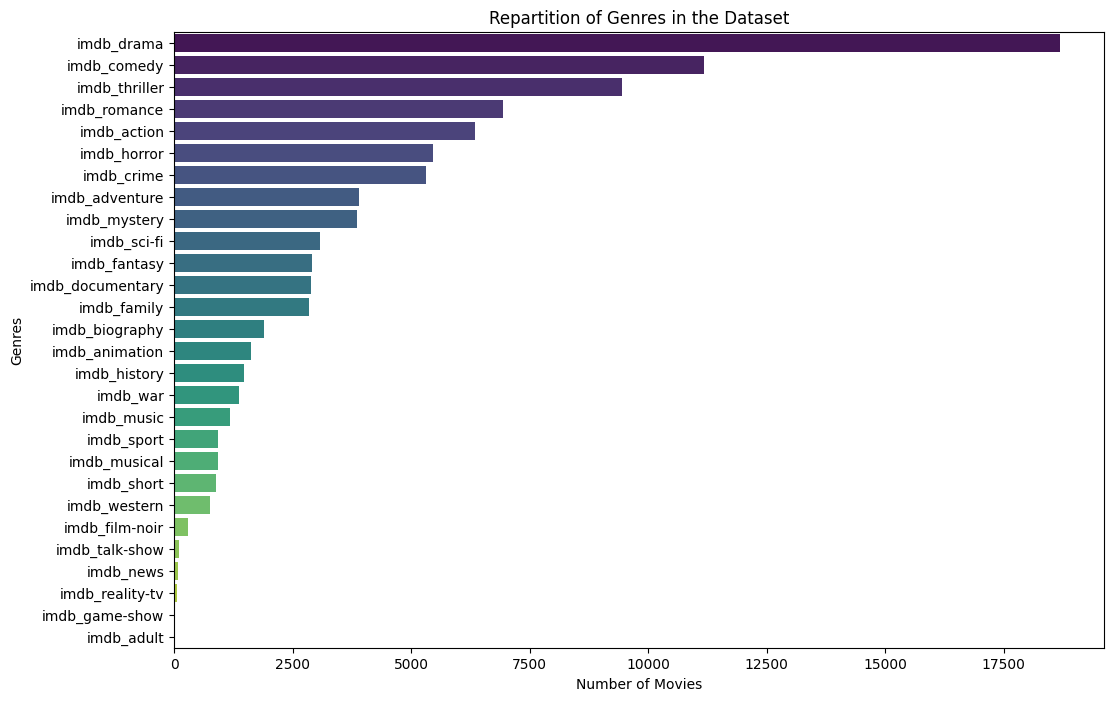
\includegraphics[width=0.8\textwidth]{img/genre}
    \caption{Répartition des genres dans le dataset}
    \label{fig:genre}
\end{figure}

\begin{figure}[H]
    \centering
    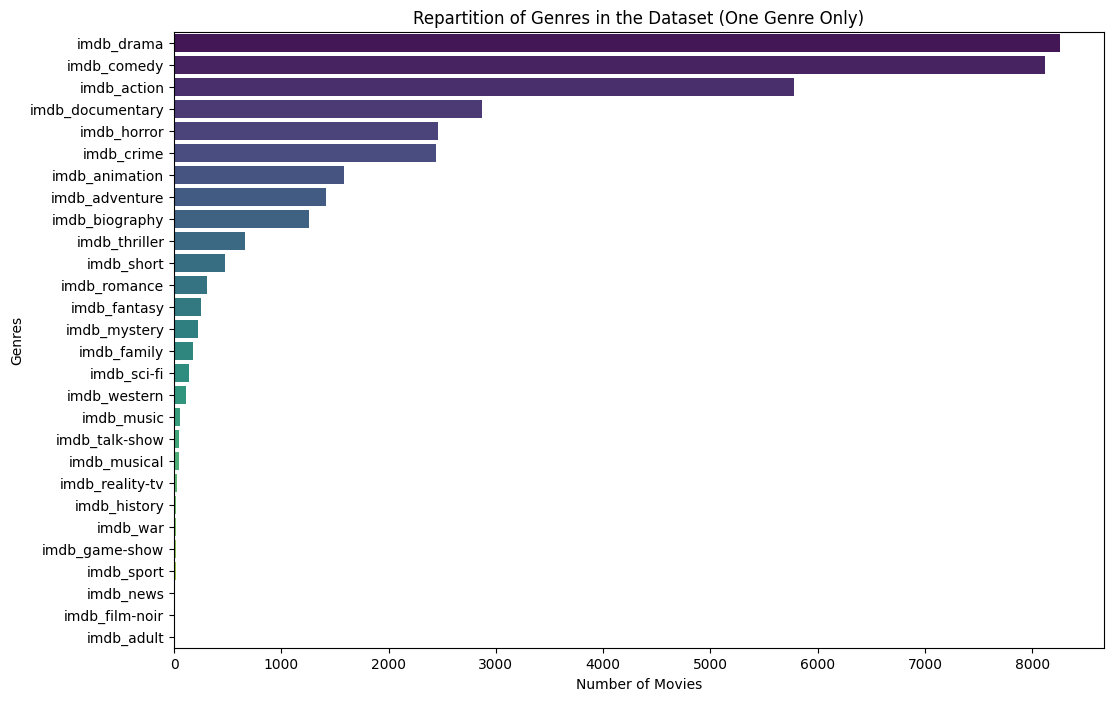
\includegraphics[width=0.8\textwidth]{img/onegenre}
    \caption{Répartition des genres dans le dataset (films avec un genre)}
    \label{fig:onegenre}
\end{figure}

\begin{figure}[H]
    \centering
    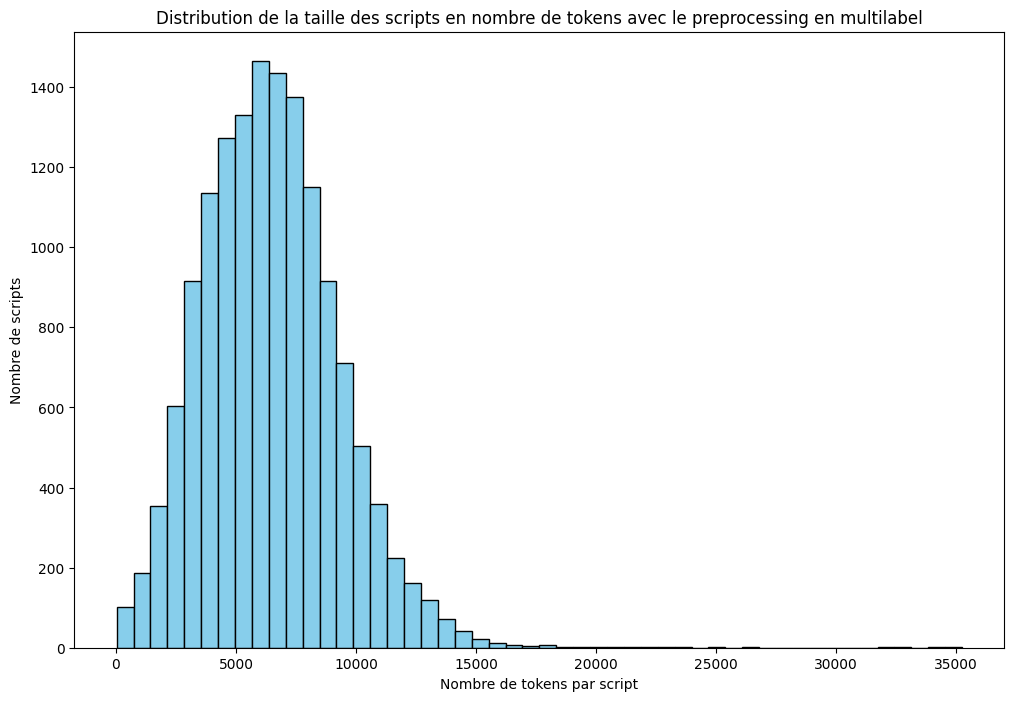
\includegraphics[width=0.9\textwidth]{img/multilabel11token}
    \caption{Distribution de la taille des scripts en nombre de tokens avec le preprocessing en multi-label}
    \label{fig:multilabel11token}
\end{figure}

\begin{figure}[H]
    \centering
    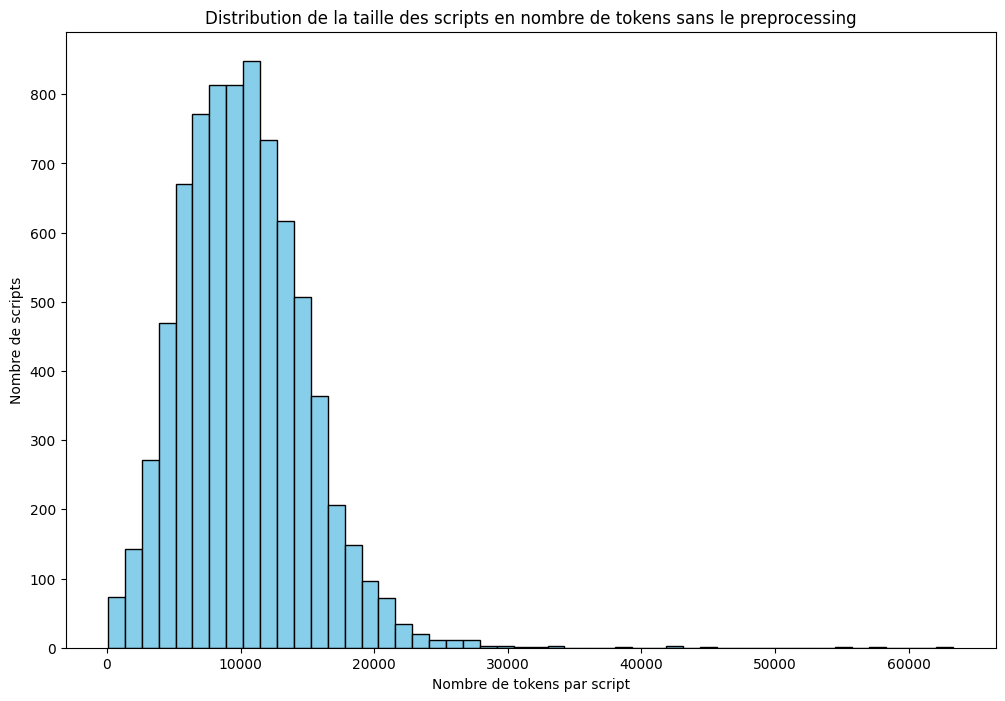
\includegraphics[width=0.9\textwidth]{img/sansprocessmulti}    
    \caption{Distribution de la taille des scripts en nombre de tokens sans le preprocessing en multi-label}
    \label{fig:sansprocessmulti}
\end{figure}

\begin{figure}[H]
    \centering
    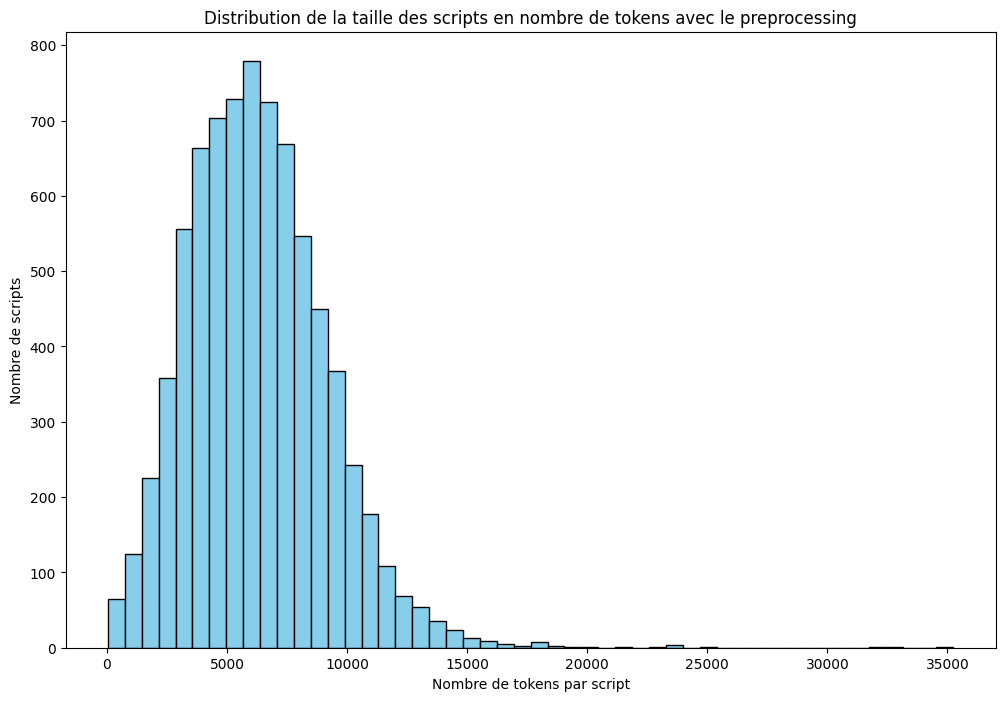
\includegraphics[width=0.9\textwidth]{img/tokenpreuni}
    \caption{Distribution de la taille des scripts en nombre de tokens avec le preprocessing multi-classe}
    \label{fig:tokenpreuni}
\end{figure}

\begin{figure}[H]
    \centering
    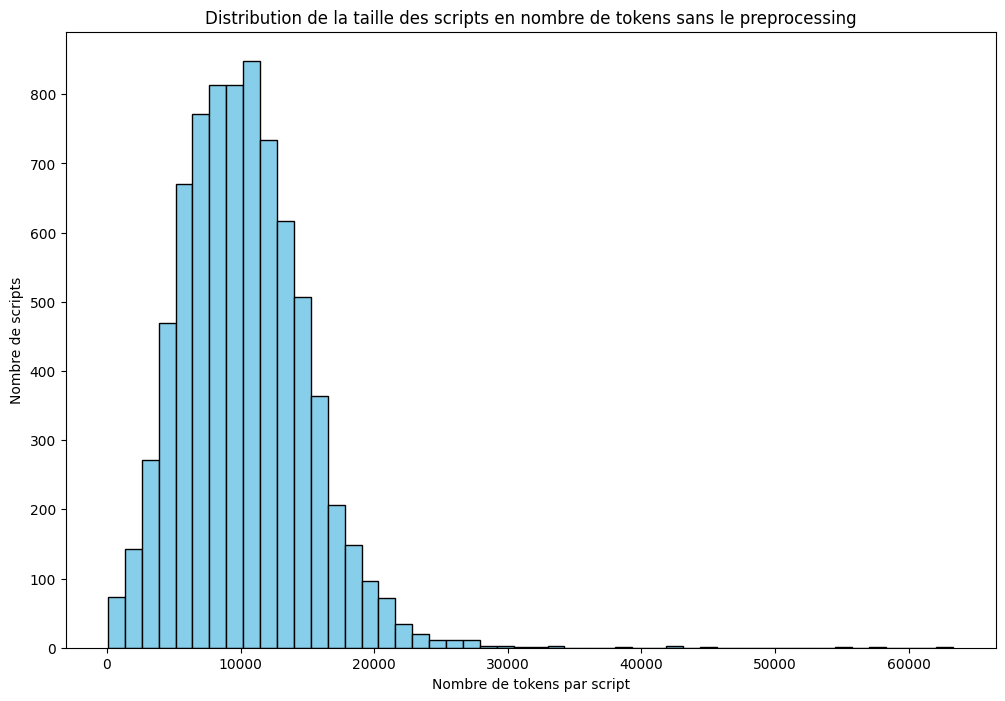
\includegraphics[width=0.9\textwidth]{img/tokensansuni}
    \caption{Distribution de la taille des scripts en nombHe de tokens sans le preprocessing en multi-classe}
    \label{fig:tokensansuni}
\end{figure}

\begin{figure}[H]
    \centering
    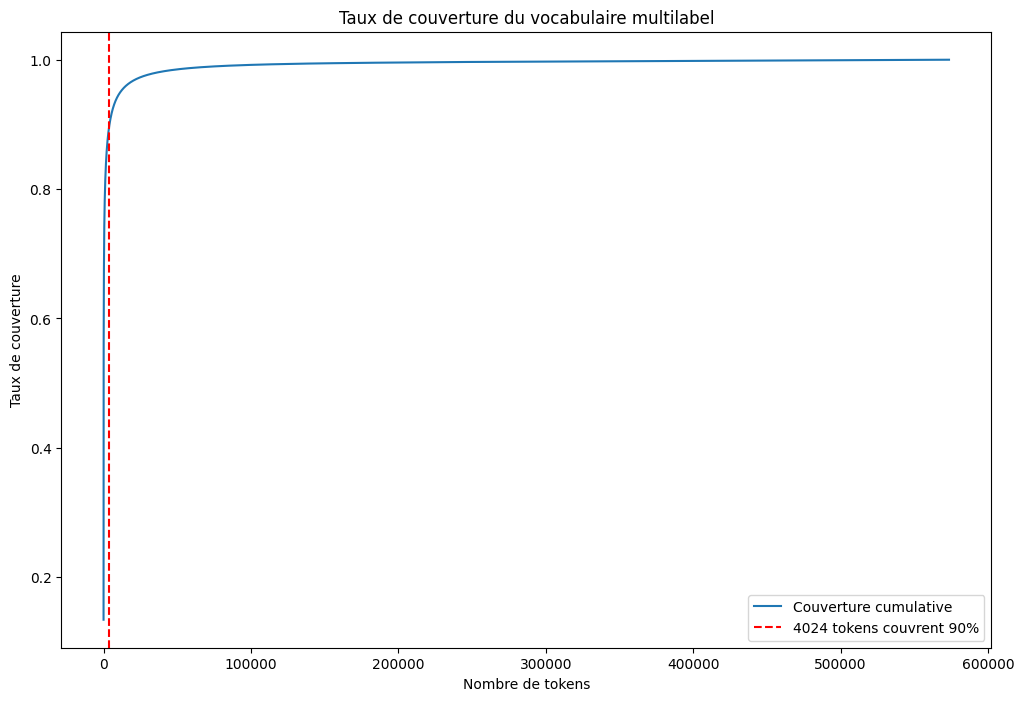
\includegraphics[width=0.9\textwidth]{img/covmulti}
    \caption{Taux de couverture du vocabulaire multi-label}
    \label{fig:covmulti}
\end{figure}

\begin{figure}[H]
    \centering
    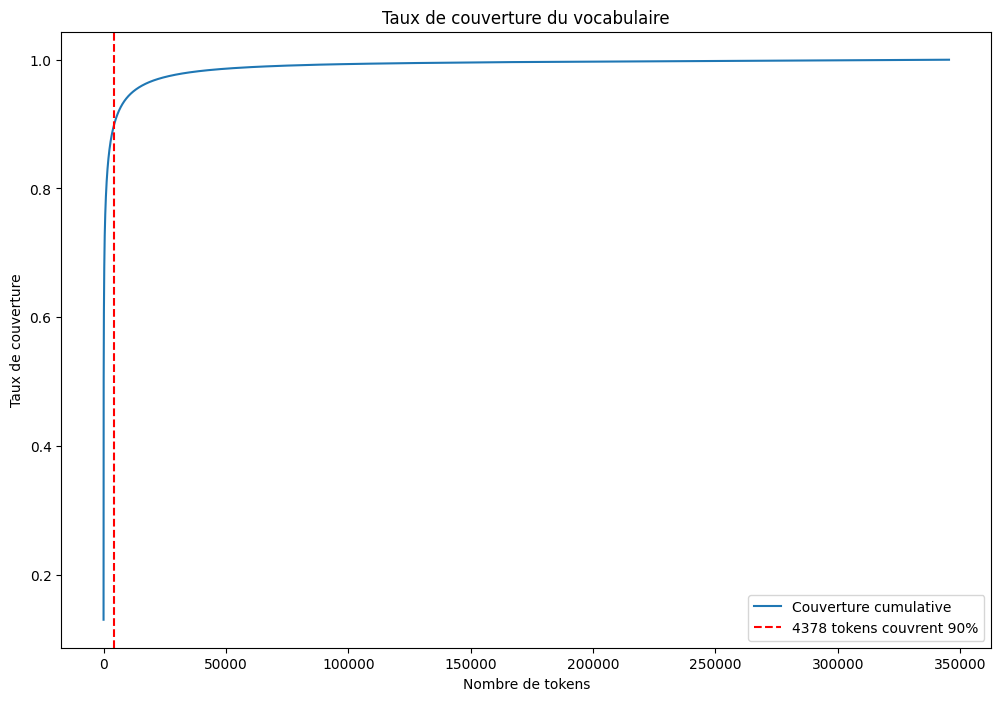
\includegraphics[width=0.9\textwidth]{img/covuni}
    \caption{Taux de couverture du vocabulaire multi-class}
    \label{fig:covuni}
\end{figure}

\begin{figure}[H]
    \centering
    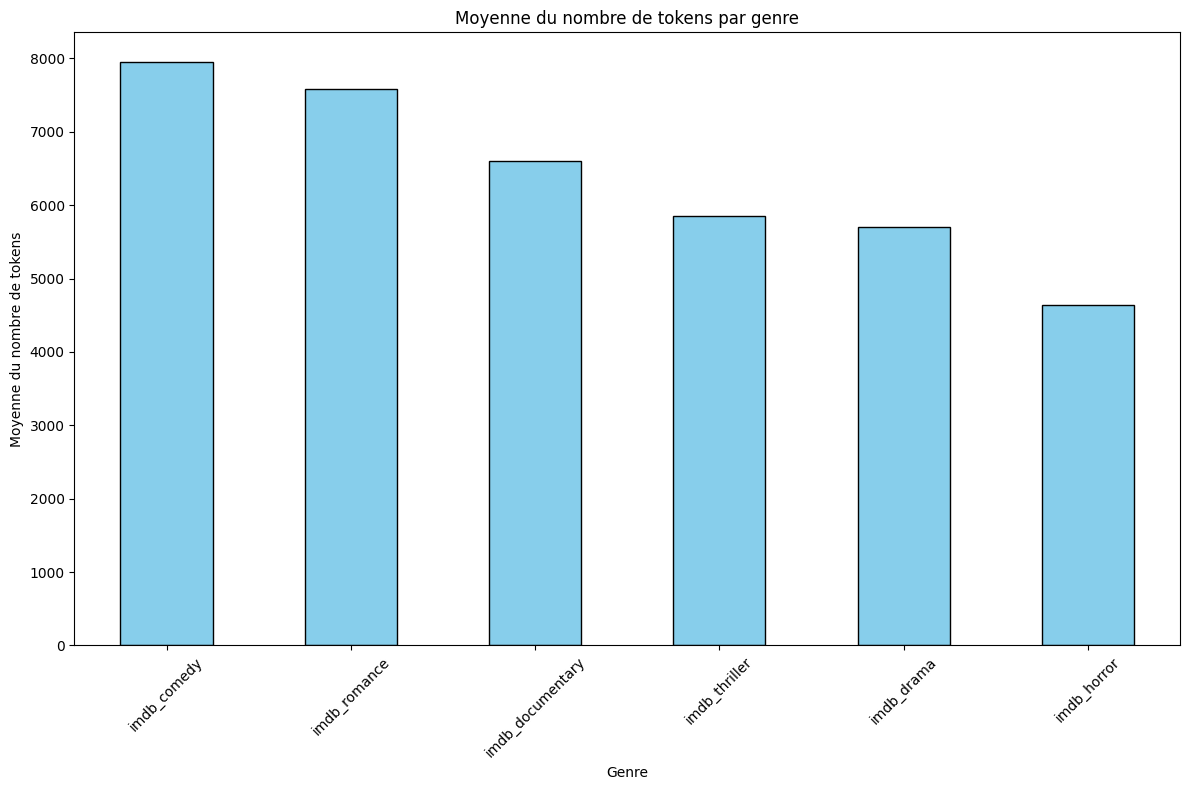
\includegraphics[width=0.9\textwidth]{img/tokNumber}
    \caption{Moyenne du nombre de tokens par genre}
    \label{fig:tok}
\end{figure}

\begin{figure}[H]
    \centering
    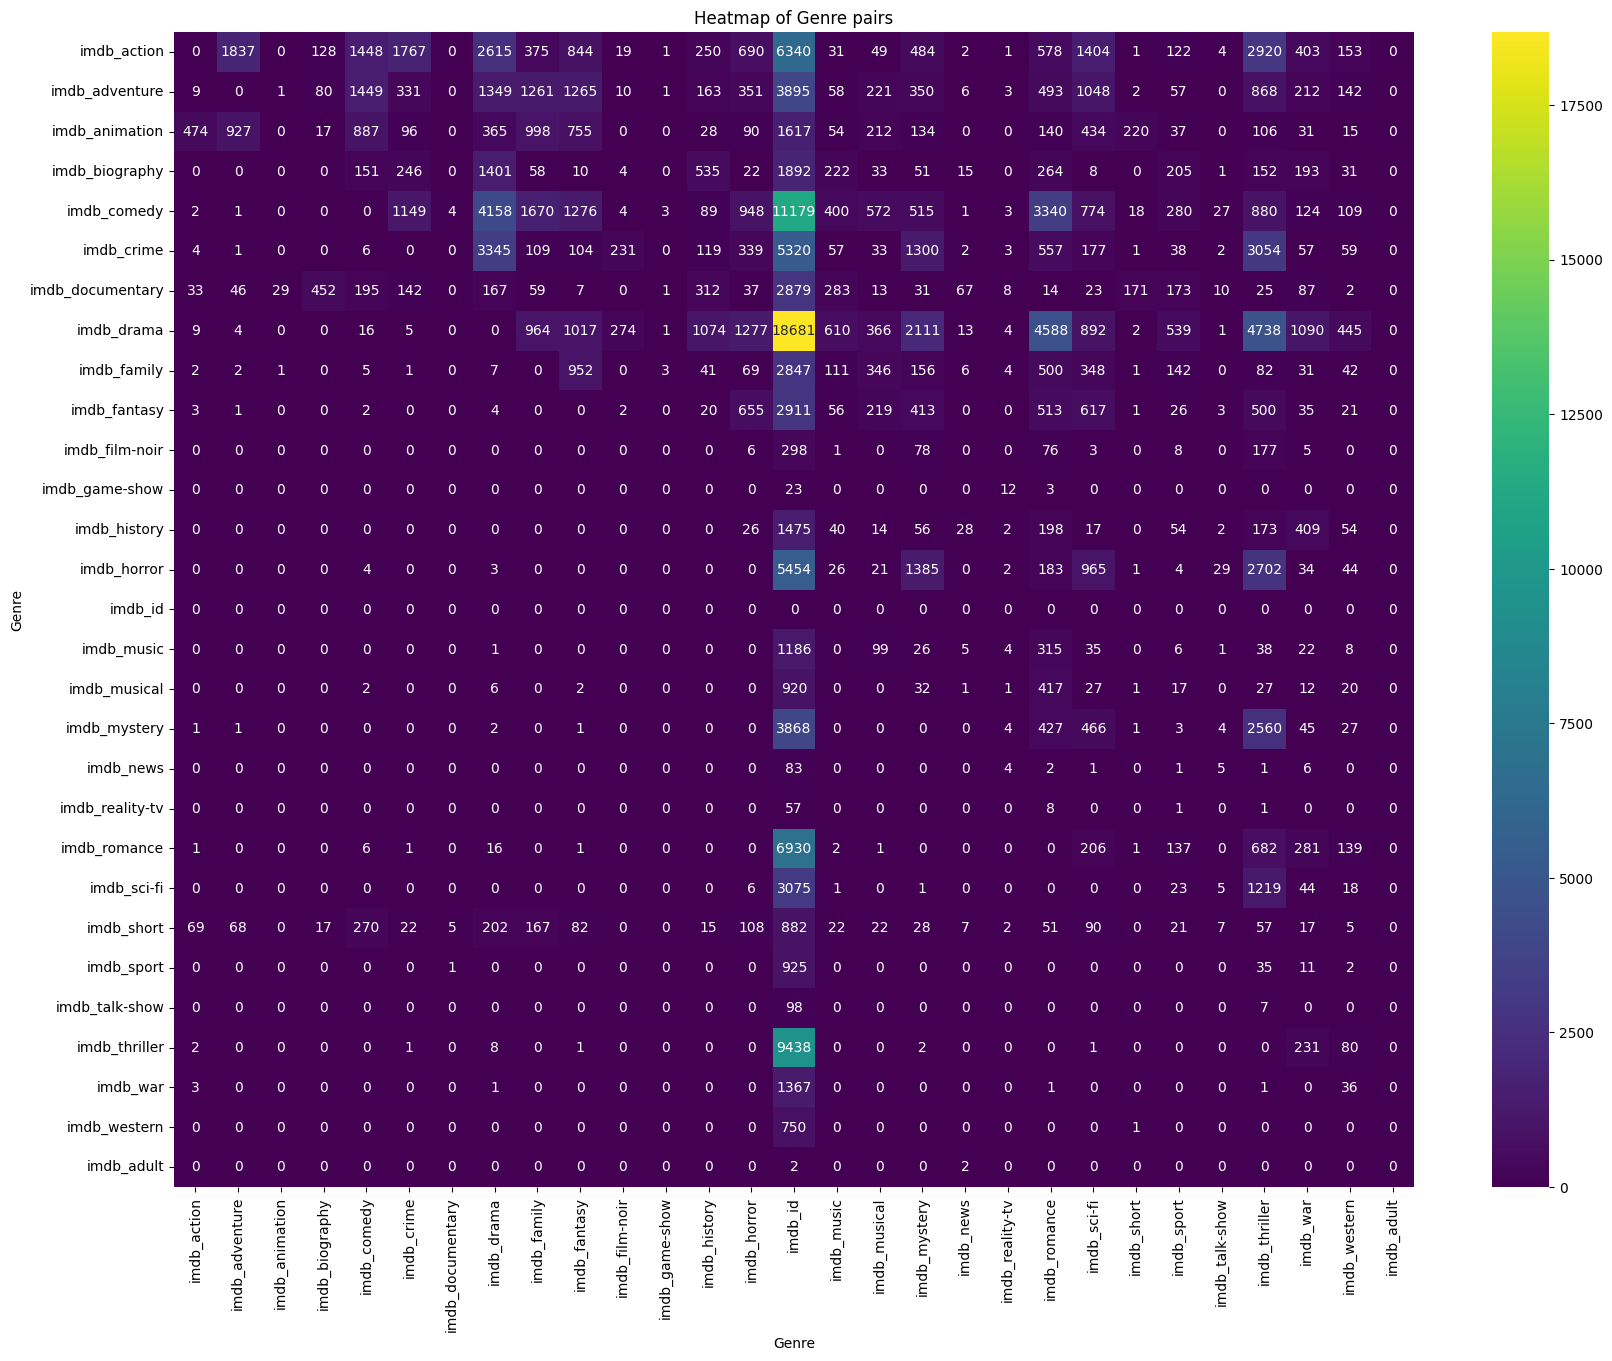
\includegraphics[width=0.9\textwidth]{img/heatmap}
    \caption{Heatmap des pairs de genres}
    \label{fig:heatmap}
\end{figure}

\begin{figure}[H]
    \centering
    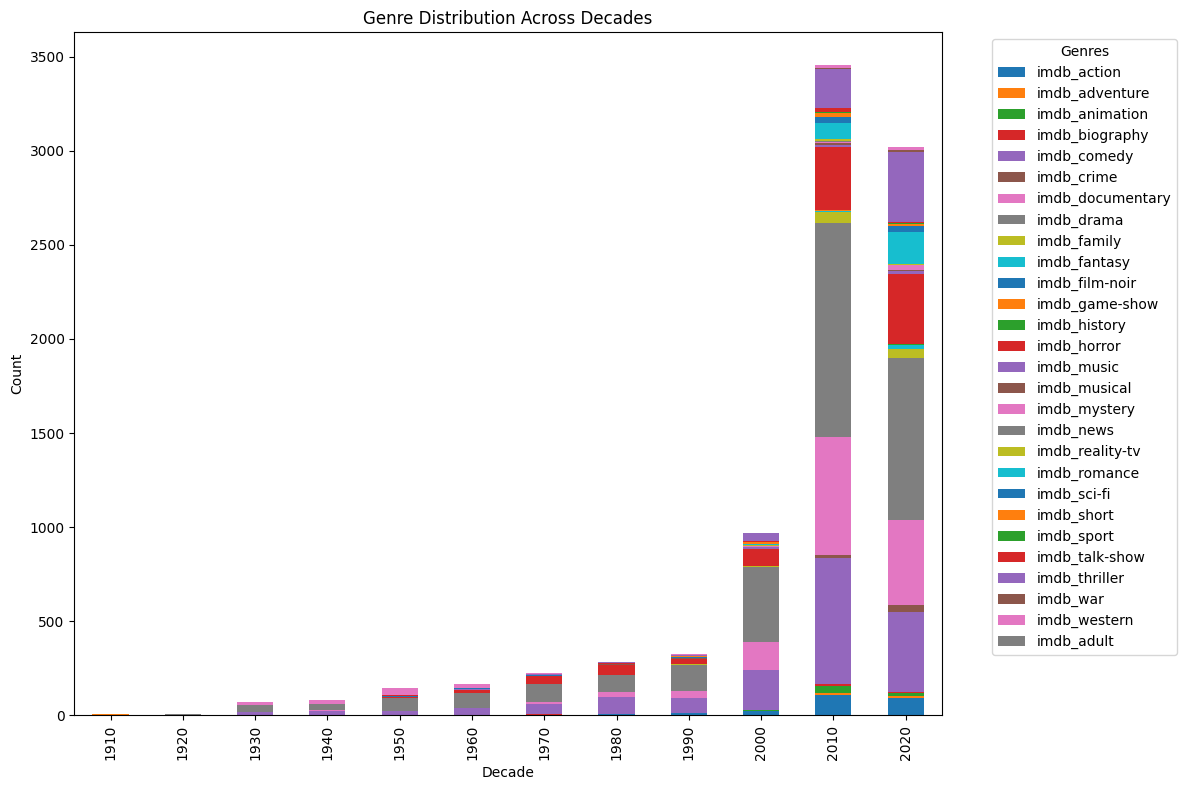
\includegraphics[width=0.9\textwidth]{img/genresdecades}
    \caption{Répartition des genres au fil des décennies}
    \label{fig:genresdecades}
\end{figure}

\begin{figure}[H]
    \centering
    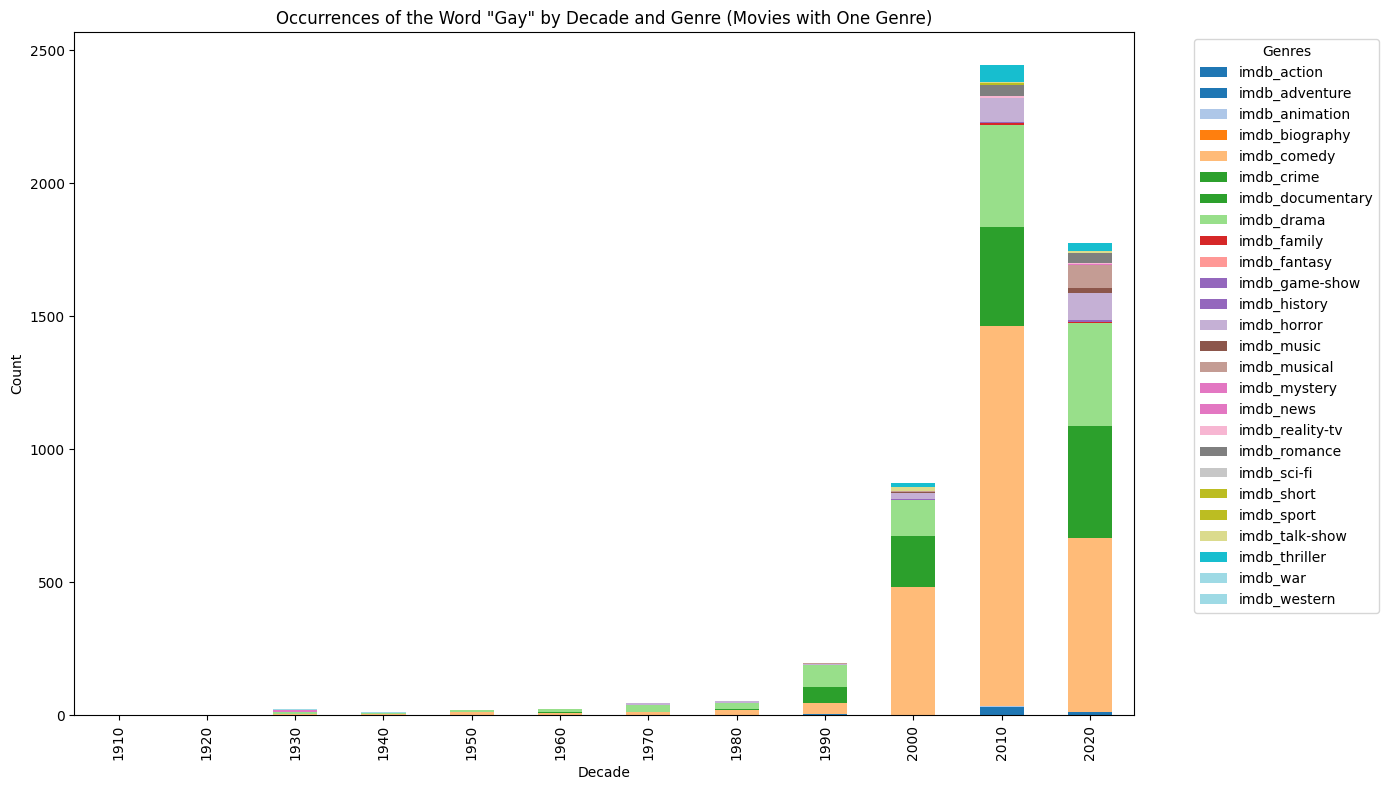
\includegraphics[width=0.9\textwidth]{img/gaydecades}
    \caption{Occurence du mot \texttt{"gay"} au fil des décennies (films avec un genre)}
    \label{fig:gaydecades}
\end{figure}

\end{document}
